\DocumentMetadata{
  lang          = en-US,
  pdfstandard   = {ua-2},
  tagging       = on,
  tagging-setup = {math/setup=mathml-SE} 
}
\documentclass{article}
\def\showanswers{0}
\def\whichlecture{}
\def\lecturetopic{}

% \documentclass{article}
\usepackage{caption}
\usepackage[pdftex]{graphicx}
\usepackage{listings}
\usepackage{tikz}
\usepackage{tikz-qtree}
\usetikzlibrary{arrows,automata}
\usetikzlibrary{shapes.geometric}
\usetikzlibrary{calc,shapes.multipart,chains,arrows}
\usepackage{amsmath}
\usepackage{amssymb}
\usepackage{amsthm}
% \usepackage{enumerate}
% \usepackage{enumitem}
\usepackage{multicol}
% \usepackage{algorithmic}
\usepackage{algorithm,caption}
\usepackage[noend]{algpseudocode}
\usepackage{fancyhdr}
\usepackage{hyperref}
\usepackage{cleveref}
\usepackage[shortlabels]{enumitem}
\usepackage{version}
\usepackage{listings, lstautogobble}
\usepackage{tcolorbox}
\usepackage{wrapfig}

\usepackage{amsmath}
% \usepackage[scaled]{helvet}
% \renewcommand\familydefault{\sfdefault} 
% \usepackage[T1]{fontenc}


\lstset {
    language=C++,
    backgroundcolor=\color{white!5}, % set backgroundcolor
    basicstyle=\footnotesize,% basic font setting
    autogobble = true,
}

\tikzstyle{vertex}=[circle,draw=black,minimum size=20pt,inner sep=0pt]
\tikzstyle{edge} = [draw,thick]
\tikzstyle{weight} = [font=\small]



\theoremstyle{definition}
\newtheorem{exercise}{Exercise}%[section]
\newtheorem{question}{Question}%[section]


%% For use with balanced BSTs
\tikzset{
itria/.style={
  draw,dashed,shape border uses incircle,
  isosceles triangle,shape border rotate=90,yshift=-1.45cm}}

\newenvironment {solution}
{
\begin{tcolorbox}
}
{
\end{tcolorbox}
}



\newcommand{\qacc}{q_{\textnormal{accept}}}
\newcommand{\qrej}{q_{\textnormal{reject}}}



\title{Unit 1B Group Problem Session}
\author{Daniel Frishberg}
\date{Cal Poly CSC 3445, Fall 2026}

\begin{document}
\lstset{upquote=true}
\setlength\parindent{0em}

\maketitle

\section{Instructions}
Solve these problems together, in a group of four.

Each team member will write up the solution to one of the questions.

Submit your solutions to Gradescope (more instructions to follow in Canvas). You will need to provide:

\begin{itemize}
    \item The names of all team members
    \item Your solutions to the problems, indicating who wrote up each solution.
    \item \textbf{You may consult generative AI tools and other sources, but do not use them to write your solutions.}
    \item Cite any external sources or tools used and you used them, or indicate that you did not use any. \textbf{This part is required.}
\end{itemize}

\pagebreak

\section{Questions}
\begin{enumerate}
\item Consider the procedure for converting a DFA to an equivalent regular expression, from class. 

Here is the initial machine:

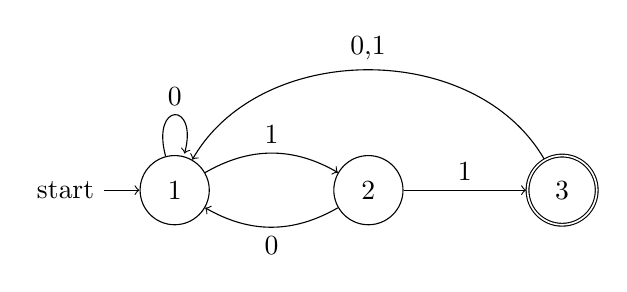
\begin{tikzpicture}[node distance=7em]
    \node[state, initial] (1) {$1$};
    \node[state, right of=1] (2) {$2$};
    \node[state, accepting, right of=2] (3) {$3$};
    \draw
      (1) edge[loop above] node{0} (1)
    (1) edge[style = ->, bend left] node [above] {1} (2)
    (3) edge[bend right=60, style = ->] node [above] {0,1} (1)
    (2) edge[style = ->, bend left] node [below] {0} (1)
    (2) edge[style = ->] node [above] {1} (3)
    ;
\end{tikzpicture}

After adding a new start and accept state, the machine is as follows:

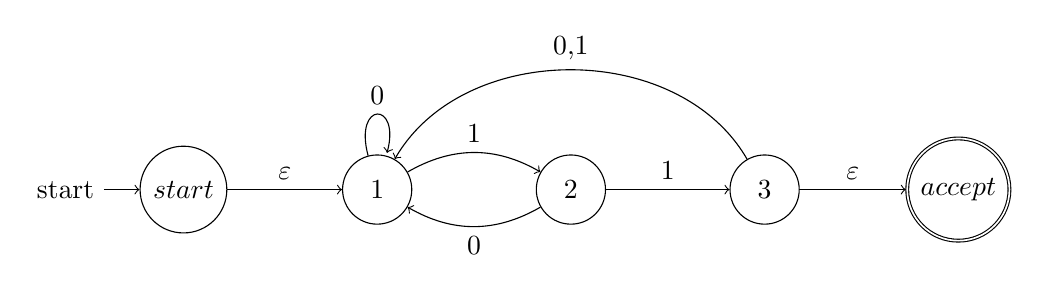
\begin{tikzpicture}[node distance=7em]
    \node[state, initial] (s) {$start$};
    \node[state, right of=s] (1) {$1$};
    \node[state, right of=1] (2) {$2$};
    \node[state, right of=2] (3) {$3$};
    \node[state, accepting, right of=3] (a) {$accept$};
    \draw 
    (s) edge[style = ->] node [above] {$\varepsilon$} (1)
    (1) edge[loop above] node{0} (1)
    (1) edge[style = ->, bend left] node [above] {1} (2)
    (3) edge[bend right=60, style = ->] node [above] {0,1} (1)
    (2) edge[style = ->, bend left] node [below] {0} (1)
    (2) edge[style = ->] node [above] {1} (3)
    (3) edge[style = ->] node [above] {$\varepsilon$} (a)
    ;
\end{tikzpicture}
     Draw the machine that results from eliminating state 1, including the regular expression(s) appearing on each new transition. Then eliminate state 2, then state 3; then write the resulting regular expression. Also write each intermediate machine.
\pagebreak
    
\item Convert the following NFA to an equivalent DFA, using the procedure from class. You do not have to draw unreachable or dead states.

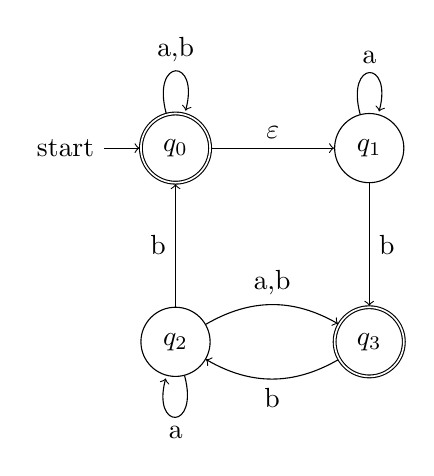
\begin{tikzpicture}[node distance=7em]
    \node[state, accepting, initial] (q0) {$q_0$};
    \node[state, right of=q0] (q1) {$q_1$};
    \node[state, below of=q0] (q2) {$q_2$};
    \node[state, accepting, right of=q2] (q3) {$q_3$};
    \draw (q0) edge[loop above] node [above ] {a,b} (q0)
    (q0) edge[style = ->] node [above] {$\varepsilon$} (q1)
    (q1) edge[loop above] node [above] {a} (q1)
    (q1) edge[style = ->] node [right] {b} (q3)
    (q2) edge[loop below] node [below] {a} (q3)
    (q2) edge[style = ->] node [left] {b} (q0)
    (q2) edge[bend left, style = ->] node [above] {a,b} (q3)
    (q3) edge[bend left, style = ->] node [below] {b} (q2);
\end{tikzpicture}

\pagebreak

\item  Let $\Sigma = \{a,b,c\}$. Prove that the language 
\[
L_1 = \{c^la^mb^{n} \mid m \geq 2n, n \geq 1, l\geq 0\}
\]

is not regular using the Pumping Lemma. 


\textbf{For reference, here is the statement of the Pumping Lemma:}


\textbf{Lemma} (Pumping Lemma):
Let $L$ be a regular language. Then there exists some number $p$ (the ``pumping length'') such that the following holds:  

Let $w$ be a string in $L$ where $|w| \geq p$. Then there exist substrings $x, y, z$ where $w = xyz$ and:
\begin{enumerate}
    \item For every $i \geq 0, xy^iz \in L$.
    \item $|y| > 0$.
    \item $|xy| \leq p$.
\end{enumerate}

\textbf{Give your proof that $L_1$ is not regular below.}
(When referring to conditions 1-3 in your proof, you do not need to rewrite the statement of each condition. You can just say "conditions 1-3 hold" at the relevant place in your proof.)

\textbf{Proof}:

\pagebreak

\item  Let $\Sigma = \{a, b, c\}$. Prove that the language 
\begin{align*}
L = \{a^mb^n \mid m \geq 2n, n \geq 0 \}
\end{align*}
is not regular, using one or more closure properties of regular languages and the fact that $L_1$ from the previous problem is not regular.

\emph{(Hint: you may need to use concatenation and find two additional regular languages, say $L_2$ and $L_3$.)}
\end{enumerate}

\end{document}